
\noindent\begin{minipage}{\textwidth}
    \begin{table}[H]
        \centering
        \caption{Hiperparâmetros e Resultados do Melhor Modelo - vgg\_v9\_AM\_opt\_aug}
        \vspace{0.2cm}
        \resizebox{\textwidth}{!}{%
            \begin{tabular}{ll | lrrr}
                \hline
                \multicolumn{2}{c|}{\textbf{Hiperparâmetros}} & \multicolumn{4}{c}{\textbf{Métricas por Classe}} \\ \hline
                \textbf{Parâmetro} & \textbf{Valor} & \textbf{Classe} & \textbf{Precisão} & \textbf{Recall} & \textbf{F1-Score} \\ \hline
    Agendador (Patience) & 4 & 31.2 & 0,6029 & 0,7257 & 0,6586 \\ 
Agendador de LR & ReduceLROnPlateau & 31.3 & 0,6125 & 0,4851 & 0,5414 \\ 
Architecture & vgg19\_bn & 31.4 & 0,4313 & 0,6429 & 0,5163 \\ 
Batch Size & 32 & 32.3 & 0,6524 & 0,7755 & 0,7086 \\ 
Data Augmentation & False & 32.4 & 1,0000 & 0,1897 & 0,3188 \\ 
Decaimento de Peso (WD) & 0,0052 & 33.3 & 0,5217 & 0,5596 & 0,5400 \\ 
Dropout & 0,5887 & 41.4 & 0,4000 & 0,1364 & 0,2034 \\ 
Função de Perda & CrossEntropyLoss & 41.5 & 0,7586 & 0,5641 & 0,6471 \\ 
Hidden Units & 512 & 42.4 & 1,0000 & 0,2206 & 0,3614 \\ 
Label Smoothing & 0,0000 & 44.4 & 1,0000 & 0,3448 & 0,5128 \\ 
\cline{3-6} 
Otimizador & SGD & \textbf{Média (Macro)} & 0,6993 & 0,4872 & 0,5252 \\ 
Taxa de Aprendizado (LR) & 2,57e-03 & \textbf{MCC} & \multicolumn{3}{c}{0,5281} \\ 
Unfreeze Layers & 6 &  & & &  \\ 
            \hline
            \end{tabular}%
        }
    \end{table}

    \begin{figure}[H]
        \centering
        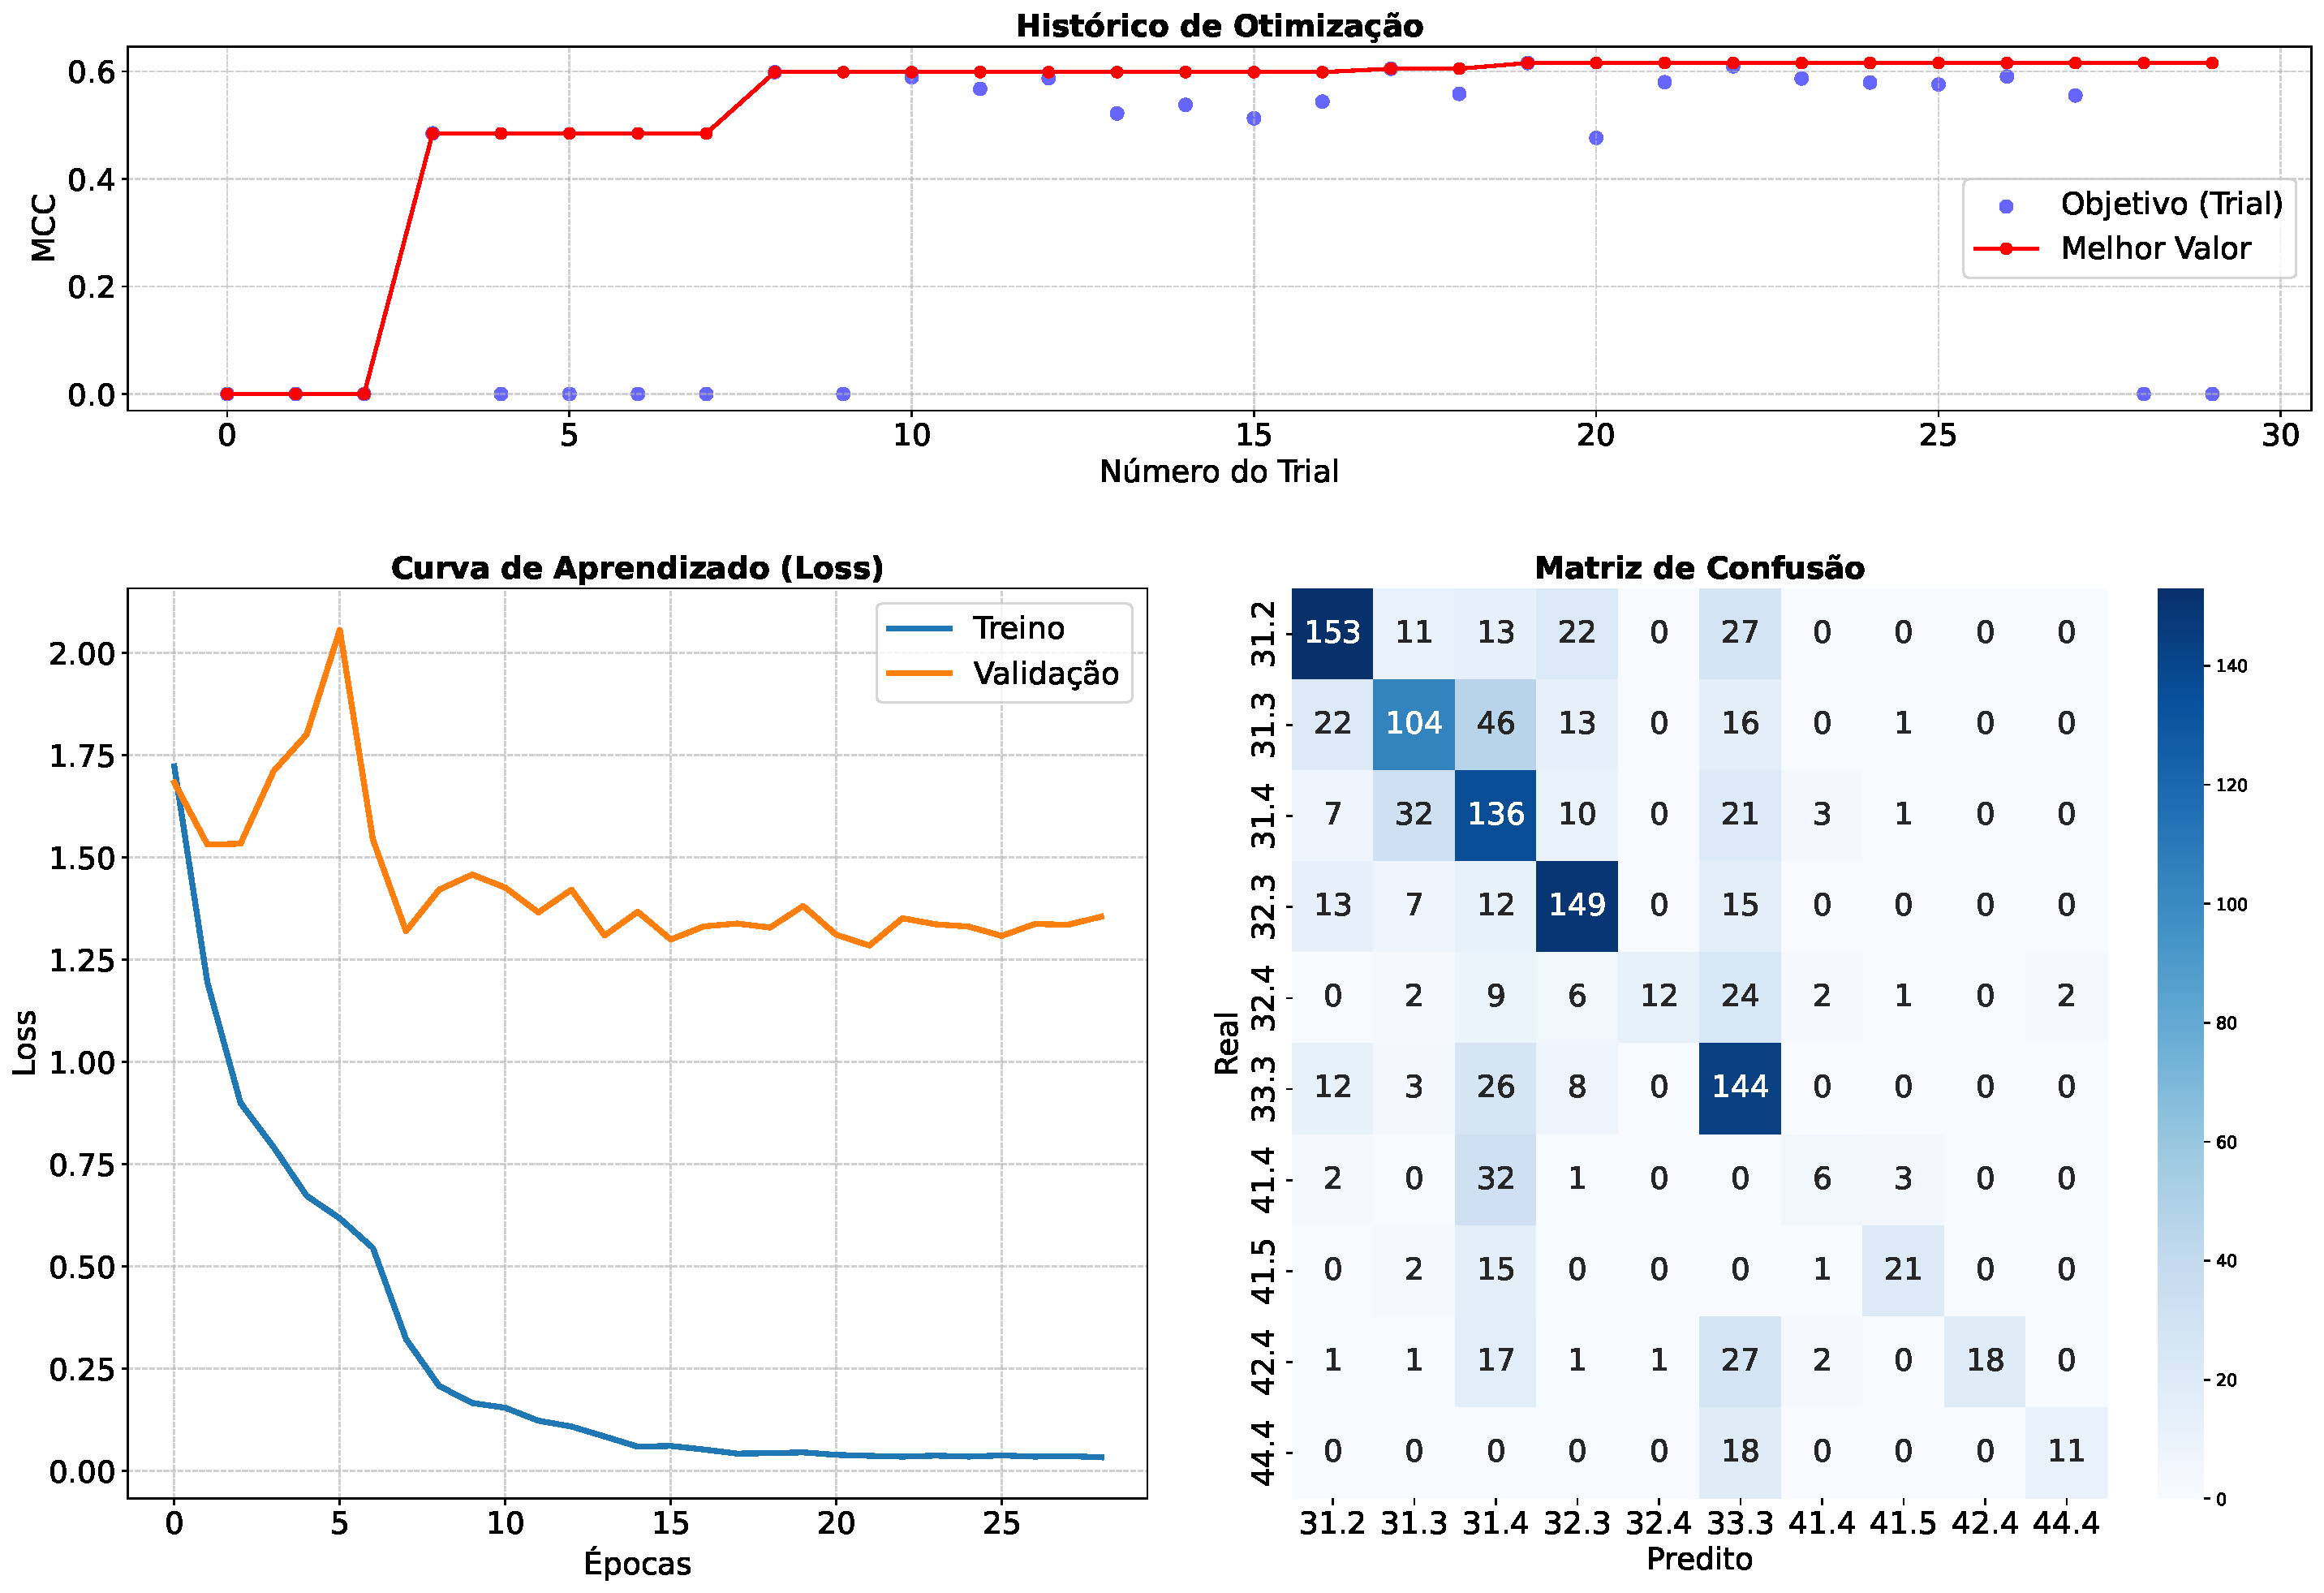
\includegraphics[width=0.85\textwidth]{tex/appendix/experiments/vgg_v9_AM_opt_aug/dashboard_consolidado.pdf}
        \caption{Histórico de Otimização, Curvas de Aprendizado e Matriz de Confusão - vgg\_v9\_AM\_opt\_aug}
    \end{figure}
\end{minipage}
\clearpage
